\documentclass[journal]{IEEEtran}

\usepackage{graphicx} % For adding images
\usepackage{amsmath} % For math equations
\usepackage{booktabs} % For better table layouts
\usepackage{enumitem} % For changing list spacing
\usepackage{float} % For exact figure placement with [H]
\usepackage{url} % For handling long URLs
\usepackage{hyperref} % For clickable hyperlinks

% Custom URL style to minimize line breaks
\urlstyle{same}
\def\UrlBreaks{\do\/\do-}

% Configure hyperref to avoid highlighting
\hypersetup{
    urlcolor=black, % URLs in black to match text
    pdfborder={0 0 0} % No border around links
}

% Document details
\title{Early Sepsis Detection with Machine Learning: Insights from MIMIC-III Data}
\author{Jesus Minjares,~\IEEEmembership{The University of Texas at Austin}}
\date{April 22, 2025}

\begin{document}

% Cover page
\begin{titlepage}
  \begin{center}
    \vspace*{0.5cm}
    % University of Texas at Austin seal
    
\includegraphics[width=0.3\textwidth]{University_of_Texas_at_Austin_Seal.png} \\
    \vspace{0.5cm}
    
    {\sffamily \Huge \textbf{Early Sepsis Detection with Machine Learning}} \\
    \vspace{0.3cm}
    {\sffamily \Large Insights from MIMIC-III Data} \\
    \vspace{1cm}
    
    \normalsize
    Research Report by \\
    \textbf{Jesus Minjares} \\
    The University of Texas at Austin \\
    \texttt{jesusminjaresjr@utexas.edu} \\
    Date: April 22, 2025 \\
    
    \vspace{1cm}
    \textbf{Additional Resources} \\
    \vspace{0.3cm}
    \begin{tabular}{p{4cm} p{10cm}}
      \toprule
      \textbf{Resource} & \textbf{Link} \\
      \midrule
      Presentation and Code & {\footnotesize \href{https://github.com/jminjares4/AI-in-Healthcare/tree/main/High_Risk_Project}{\url{https://github.com/jminjares4/AI-in-Healthcare/tree/main/High_Risk_Project}}} \\
      Video Presentation & {\footnotesize \href{https://utexas.hosted.panopto.com/Panopto/Pages/Viewer.aspx?id=2336ffb3-4ae8-47af-bb7f-b2c4016a75ec}{\url{https://utexas.hosted.panopto.com/Panopto/Pages/Viewer.aspx?id=2336ffb3-4ae8-47af-bb7f-b2c4016a75ec}}} \\
      \bottomrule
    \end{tabular}
    
    \vspace{0.5cm}
  \end{center}
\end{titlepage}

% Title and summary
\maketitle

\begin{abstract}
Sepsis, a life-threatening condition with a mortality rate of approximately 30\%, underscores the importance of early identification to enhance patient outcomes. This study developed a machine learning framework that integrates clinical notes and vital signs from the MIMIC-III database. Text data from medical notes were processed using BioBERT, and two models, LSTM and Logistic Regression, were trained, achieving an AUROC of 0.737. Significant predictors, such as heart rate and references to infection, were identified; however, further refinement is required to improve predictive accuracy and ensure equitable performance across diverse patient groups. Recent research highlights the potential of machine learning in sepsis prediction, yet challenges persist due to inconsistent clinical data. Future efforts will prioritize real-time monitoring and equitable model performance across varied populations.
\end{abstract}

\begin{IEEEkeywords}
Sepsis detection, machine learning, BioBERT, LSTM, fairness evaluation
\end{IEEEkeywords}

\section{Introduction}
Sepsis arises from an excessive immune response to infection, resulting in organ dysfunction and a substantial risk of mortality. In the United States, it affects 1.7 million adults annually, contributing to 270,000 deaths and incurring healthcare costs exceeding \$62 billion \cite{singer2016sepsis, paoli2018epidemiology}. Timely detection is critical, as each hour of delayed treatment increases mortality risk by 7.6\% \cite{kumar2006duration}. Conventional approaches, such as qSOFA and SIRS, fail to identify up to 30\% of cases due to limited sensitivity \cite{zhou2025interpretable}. To address this challenge, a machine learning framework was developed using the MIMIC-III dataset, integrating vital signs and clinical notes. By employing BioBERT and LSTM models, this study seeks to enhance prediction accuracy and promote fairness across patient demographics, facilitating prompt interventions and reducing mortality.

\section{Related Work}
Advancements in machine learning for sepsis prediction have informed this research. Yadgarov et al. (2024) reviewed 36 studies, observing that neural networks and decision trees frequently achieved AUROC scores above 0.80, surpassing traditional metrics like SOFA \cite{yadgarov2024early}. They highlighted inconsistent data quality as a persistent challenge, a difficulty also encountered in this study. Hu et al. (2024) evaluated COMPOSER, a deep-learning model implemented in emergency departments, which enhanced treatment protocols and reduced in-hospital mortality through a Best Practice Advisory system, though further validation is required \cite{hu2024impact}. Zhou et al. (2025) proposed an interpretable model for sepsis risk assessment at triage using MIMIC-IV, attaining an AUROC of 0.83 with Gradient Boosting and emphasizing detailed triage data \cite{zhou2025interpretable}. This study distinguishes itself by incorporating clinical notes and prioritizing fairness, addressing disparities in equitable care and real-time applicability.

\section{Methodology}
The MIMIC-III dataset, encompassing vital signs (CHARTEVENTS), clinical notes (NOTEEVENTS), diagnoses (DIAGNOSES\_ICD), and patient demographics (PATIENTS), served as the data source. The methodology comprised four phases:

\begin{enumerate}[itemsep=0pt,parsep=2pt]
    \item \textbf{Data Acquisition}: Vital signs, clinical notes, diagnoses, and patient information were collected from MIMIC-III.
    \item \textbf{Data Preprocessing}: Vital signs, including heart rate, blood pressure, and respiratory rate, were aggregated into 12-hour intervals. Missing values were imputed using the last observed value or the dataset mean. Clinical notes were analyzed for terms such as “infection” and converted into BioBERT embeddings. Sepsis labels were derived from ICD9 codes.
    \item \textbf{Model Development}: Logistic Regression and LSTM models were trained over five epochs. The LSTM architecture included 64 units, a 32-unit dense layer, and a sigmoid activation function.
    \item \textbf{Performance Evaluation}: Models were assessed using AUROC, precision, recall, and F1 scores. Fairness across male and female patients was examined, and SHAP values identified the most influential features.
\end{enumerate}

\section{Results}
The LSTM model achieved an AUROC of 0.737, marginally outperforming Logistic Regression’s 0.722, as depicted in the ROC curves in Figure \ref{fig:roc}. Confusion matrices in Figure \ref{fig:cm} indicate that the LSTM accurately classified 24,233 non-sepsis cases but failed to detect 16,432 sepsis cases, whereas Logistic Regression missed fewer sepsis cases (10,981) but generated 8,335 false positives. Precision-recall curves in Figure \ref{fig:pr-curves} reveal that Logistic Regression exhibited higher precision at lower recall, while LSTM performed better at higher recall. Fairness analysis in Figure \ref{fig:fairness} shows comparable AUROC scores (0.731 for females, 0.743 for males), yet recall was higher for females (0.197) than males (0.172), suggesting potential bias. SHAP analysis in Figure \ref{fig:shap} identified heart rate (SHAP values up to 0.2), infection mentions (up to 0.8), and fever (up to 0.1) as primary predictors. Vital sign distributions in Figure \ref{fig:dist} demonstrate that sepsis patients exhibited elevated heart rates (100–120 bpm versus 80–100 for non-sepsis), lower blood pressure (occasionally under 80 mmHg versus 80–100), and higher respiratory rates (20–25 breaths/min versus 15–20). BioBERT embeddings are visualized in Figure \ref{fig:biobert_heatmap}, with t-SNE analysis in Figure \ref{fig:tsne} revealing clusters (e.g., Notes 2 and 23) reflecting similar clinical note patterns. Training metrics in Figure \ref{fig:curves} indicate that the LSTM attained a training accuracy of 0.7505 and validation accuracy of 0.7495, with training and validation losses of 0.500 and 0.502, respectively. These findings underscore the framework’s potential for early sepsis detection, though further improvements in accuracy and fairness are necessary.

\begin{figure}[ht]
    \centering
    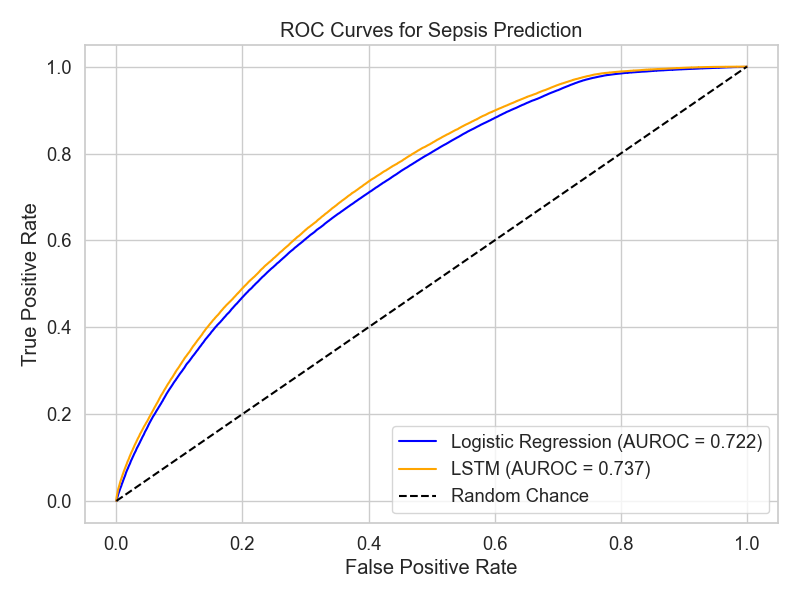
\includegraphics[width=0.8\columnwidth]{roc_curves.png}
    \caption{ROC Curves for Sepsis Prediction (LSTM: AUROC 0.737, Logistic Regression: AUROC 0.722).}
    \label{fig:roc}
\end{figure}

\begin{figure}[ht]
    \centering
    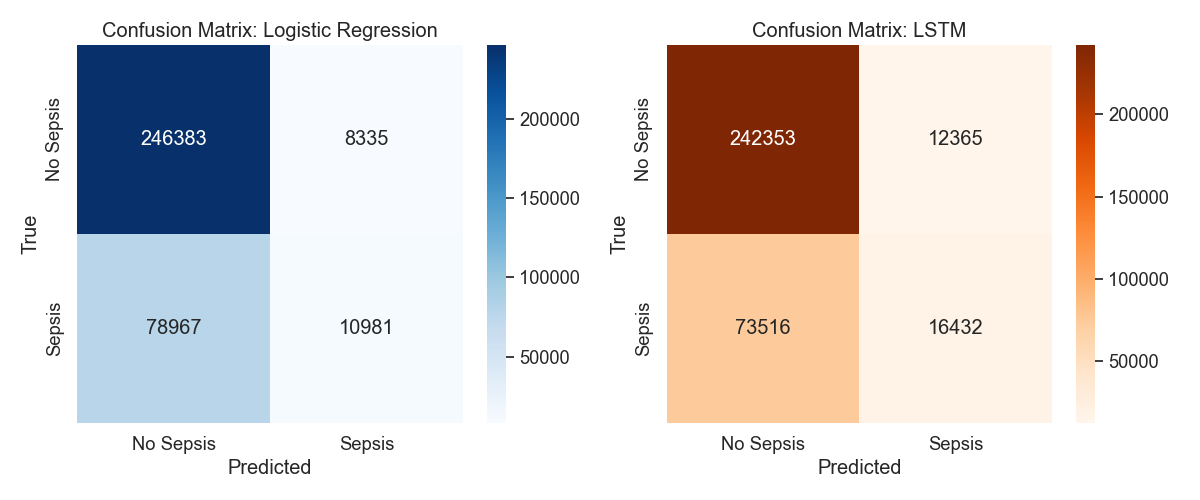
\includegraphics[width=0.8\columnwidth]{confusion_matrices.png}
    \caption{Confusion Matrices for Sepsis Prediction. Logistic Regression: 24,683 true negatives, 10,981 false negatives; LSTM: 24,233 true negatives, 16,432 false negatives.}
    \label{fig:cm}
\end{figure}

\begin{figure}[ht]
    \centering
    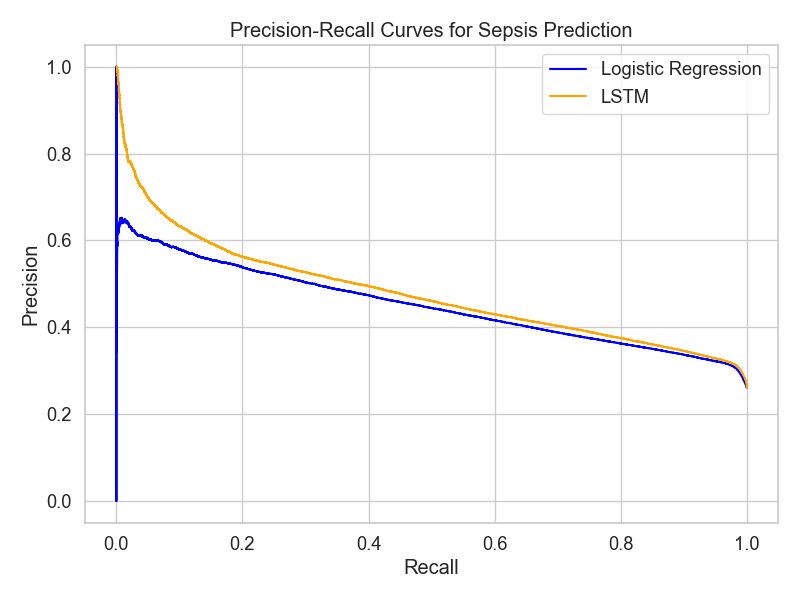
\includegraphics[width=0.8\columnwidth]{precision_recall_curves.png}
    \caption{Precision-Recall Curves for Sepsis Prediction.}
    \label{fig:pr-curves}
\end{figure}

\begin{figure}[ht]
    \centering
    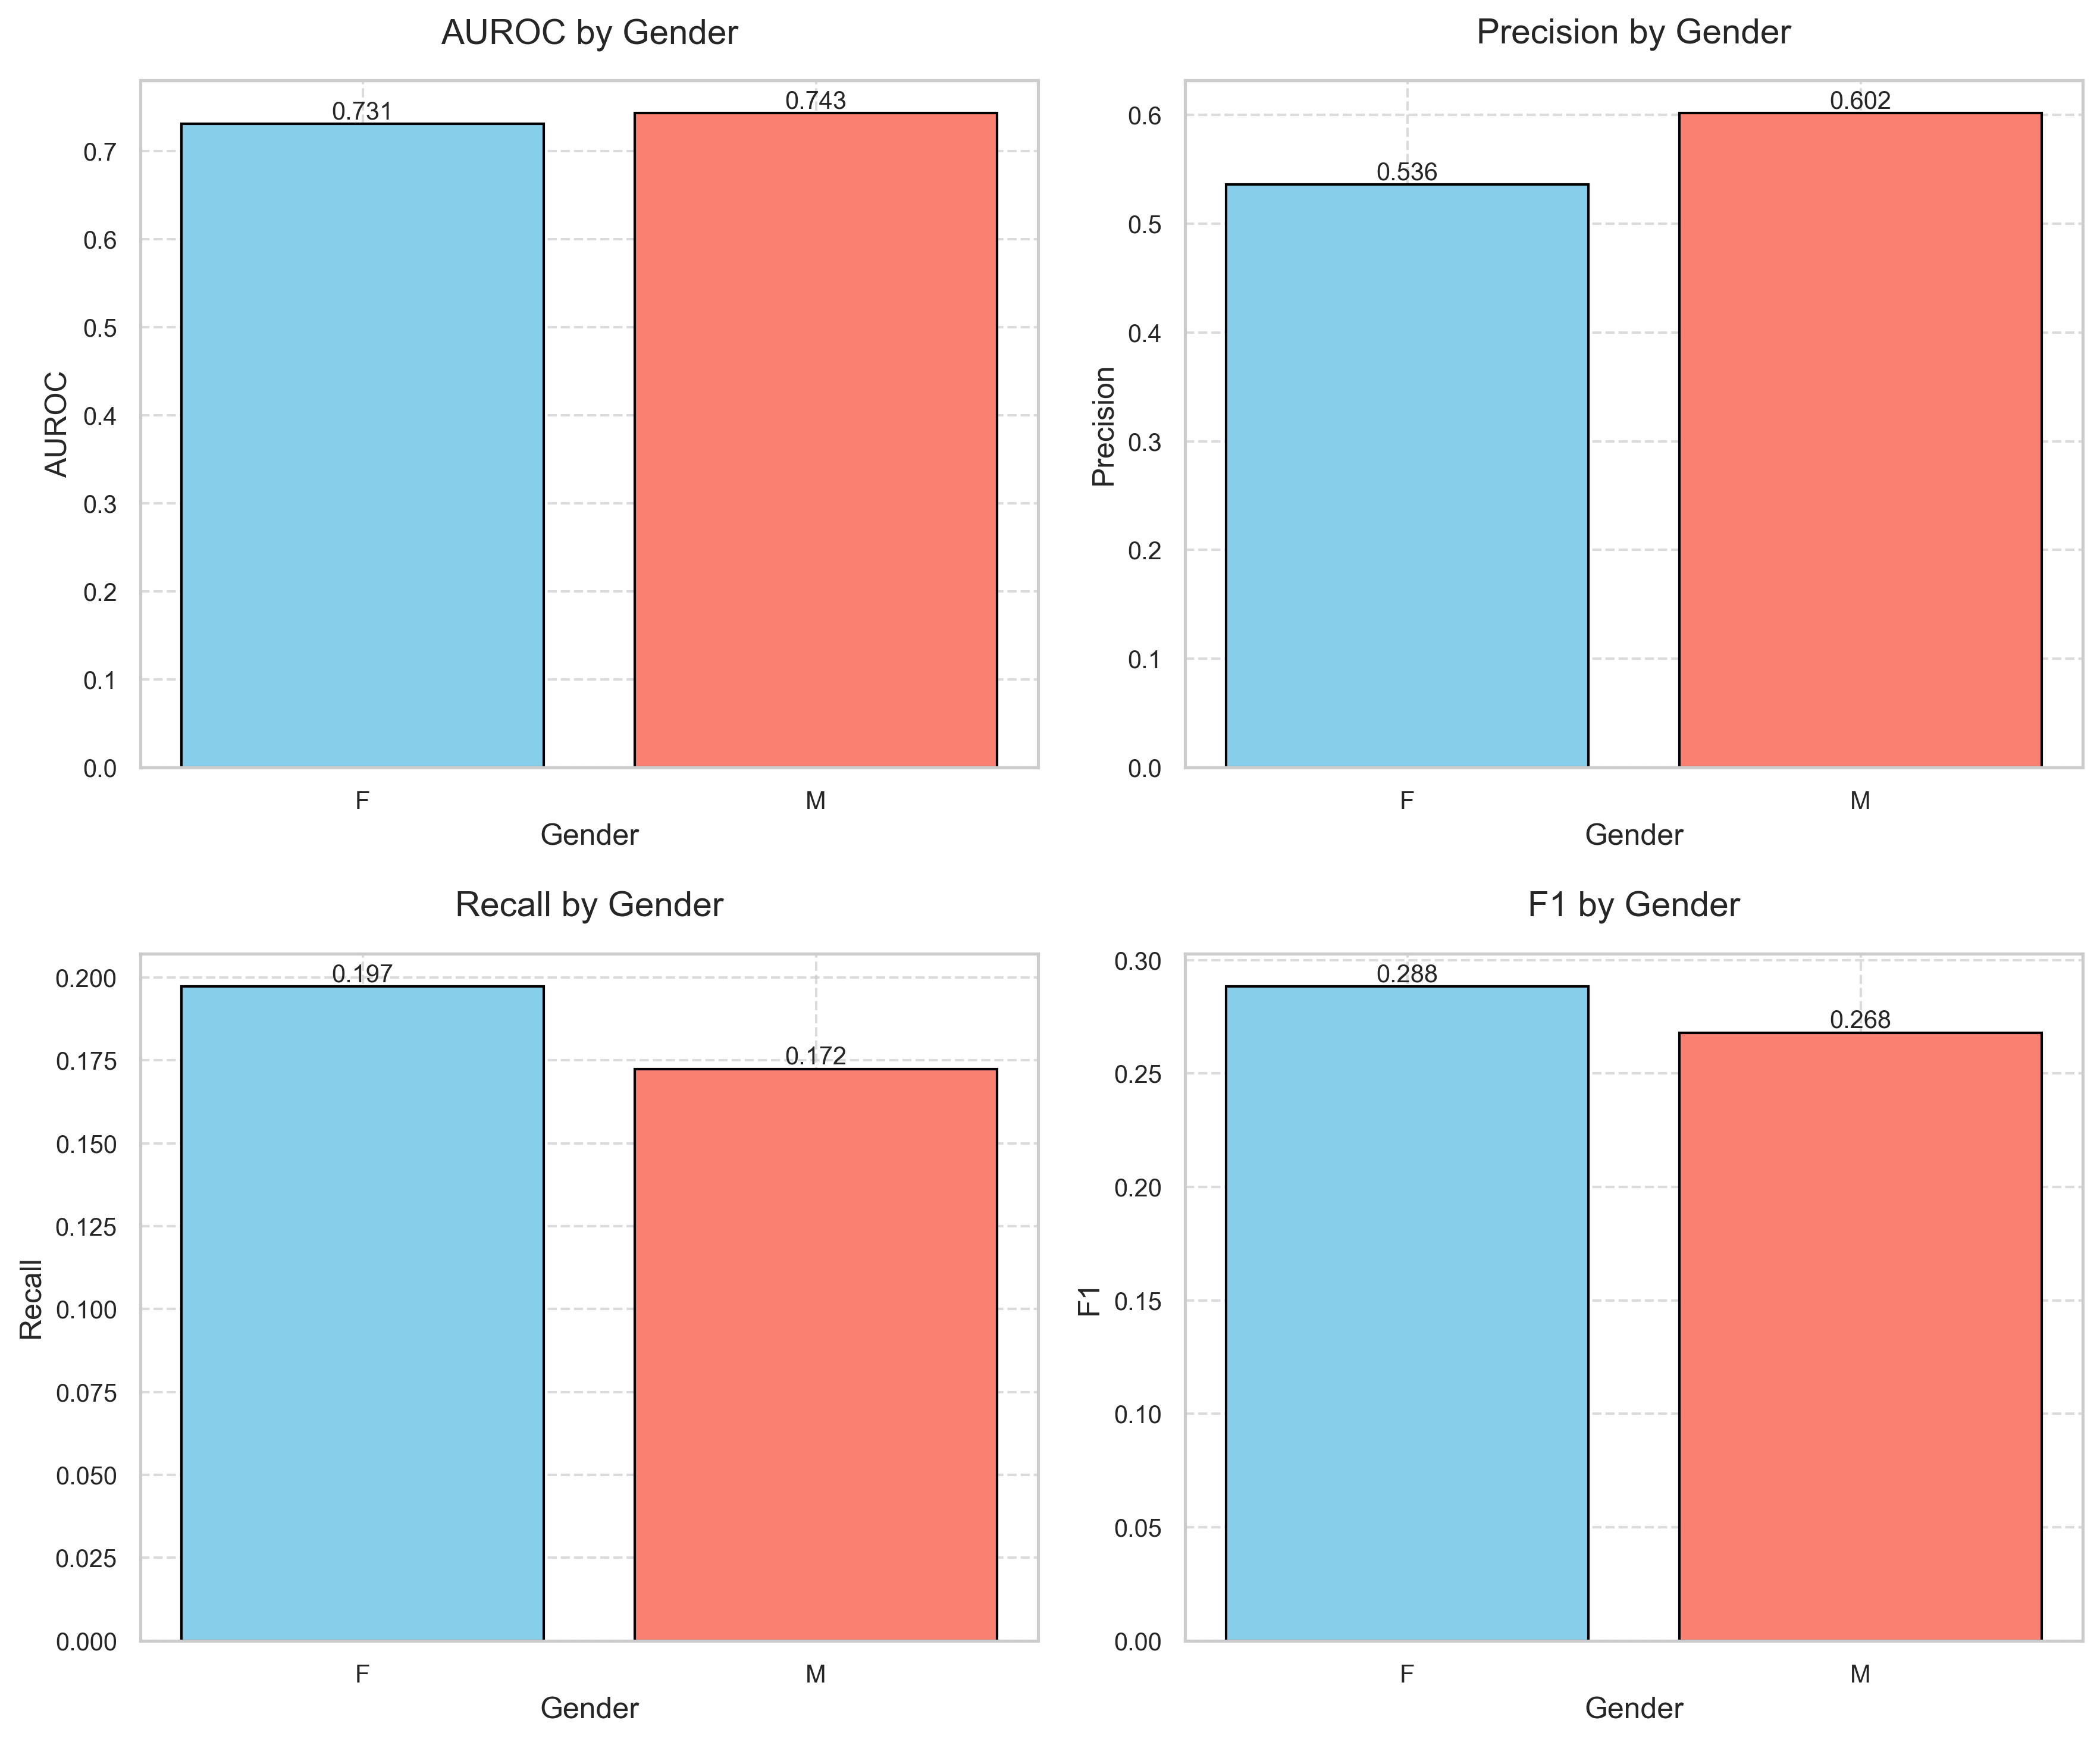
\includegraphics[width=0.8\columnwidth]{fairness_metrics.png}
    \caption{Fairness Metrics by Gender. AUROC: Female 0.731, Male 0.743; Recall: Female 0.197, Male 0.172.}
    \label{fig:fairness}
\end{figure}

\begin{figure}[H]
    \centering
    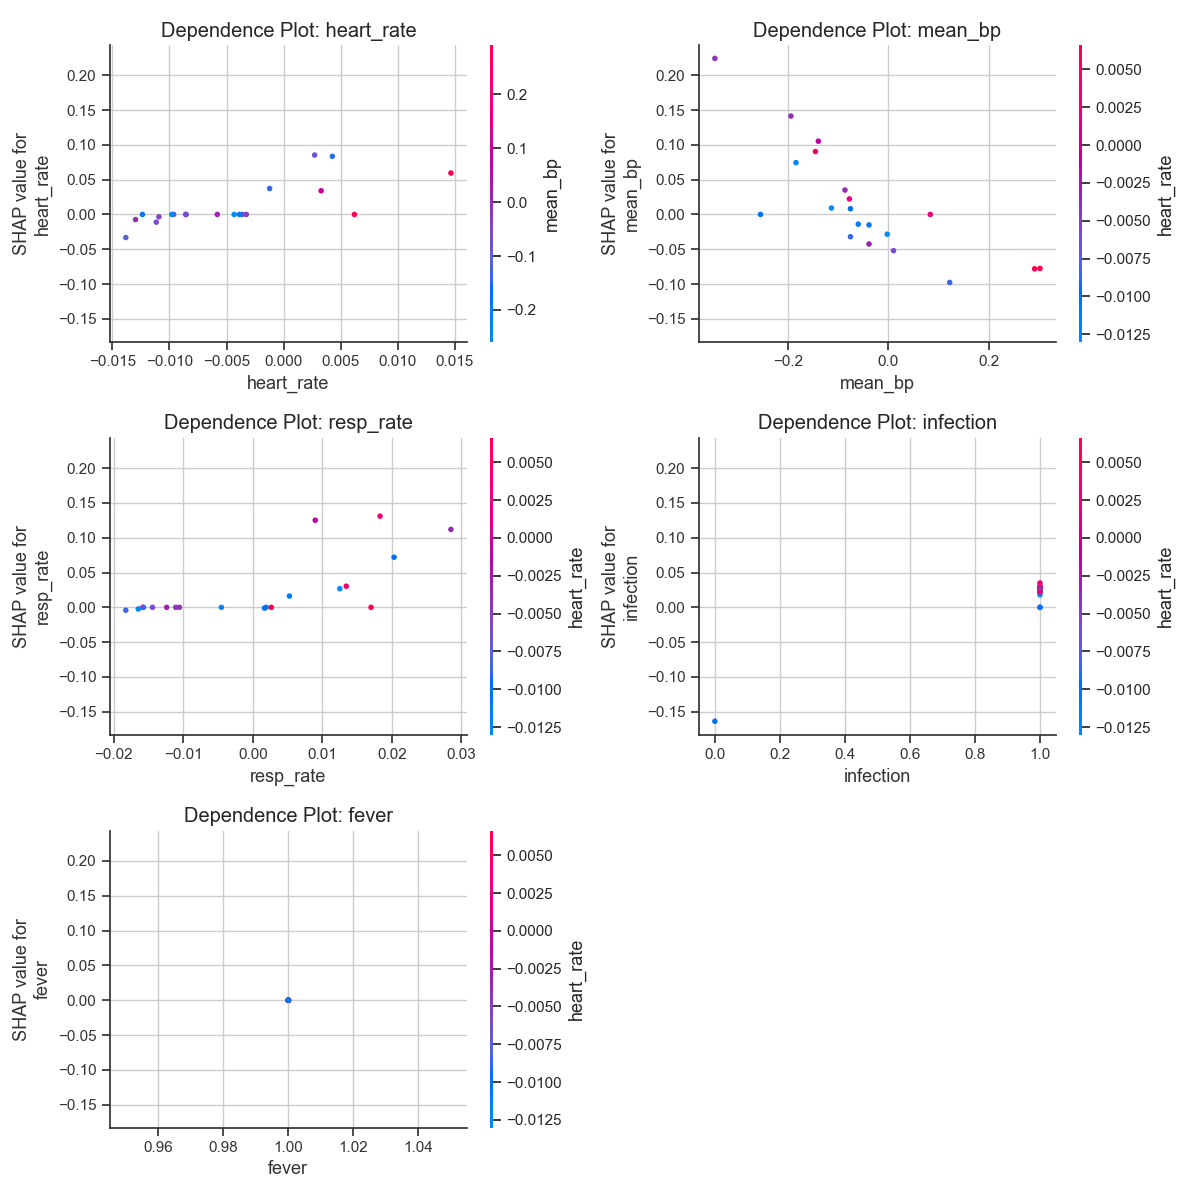
\includegraphics[width=0.8\columnwidth]{shap_dependence_combined.png}
    \caption{SHAP Dependence Plots. Heart Rate: SHAP values up to 0.2; Infection: SHAP values up to 0.8; Fever: SHAP values up to 0.1.}
    \label{fig:shap}
\end{figure}

\begin{figure}[H]
    \centering
    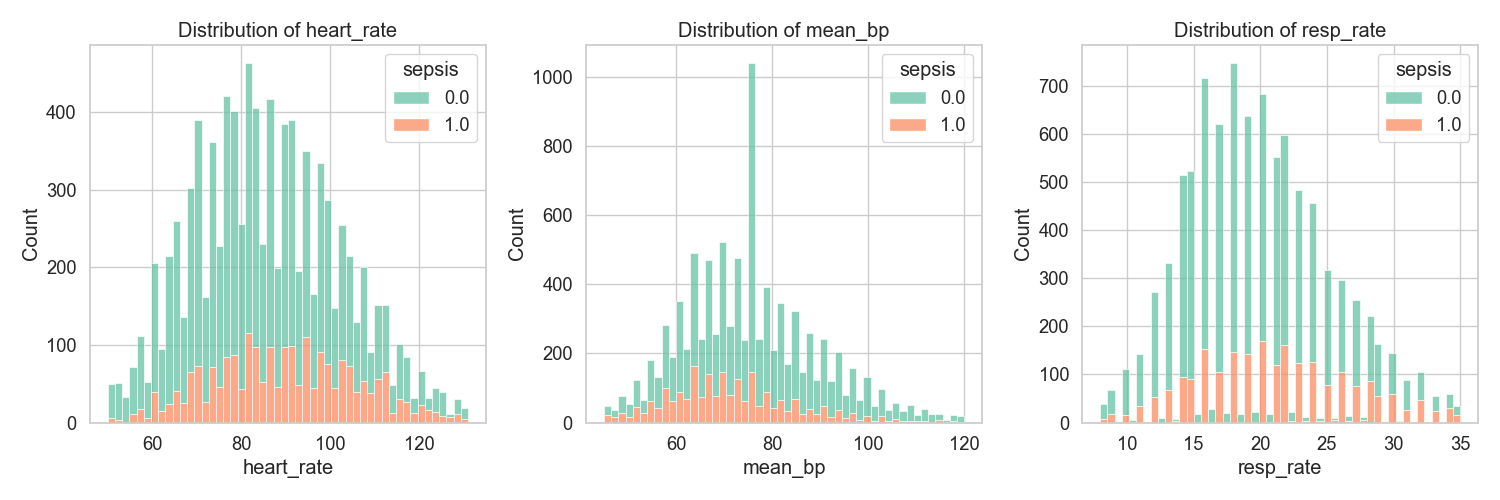
\includegraphics[width=0.8\columnwidth]{feature_distributions.png}
    \caption{Vital Sign Patterns. Heart Rate: Sepsis 100–120 bpm, Non-Sepsis 80–100 bpm; Blood Pressure: Sepsis some <80 mmHg, Non-Sepsis 80–100 mmHg; Breathing Rate: Sepsis 20–25 breaths/min, Non-Sepsis 15–20 breaths/min.}
    \label{fig:dist}
\end{figure}

\begin{figure}[H]
    \centering
    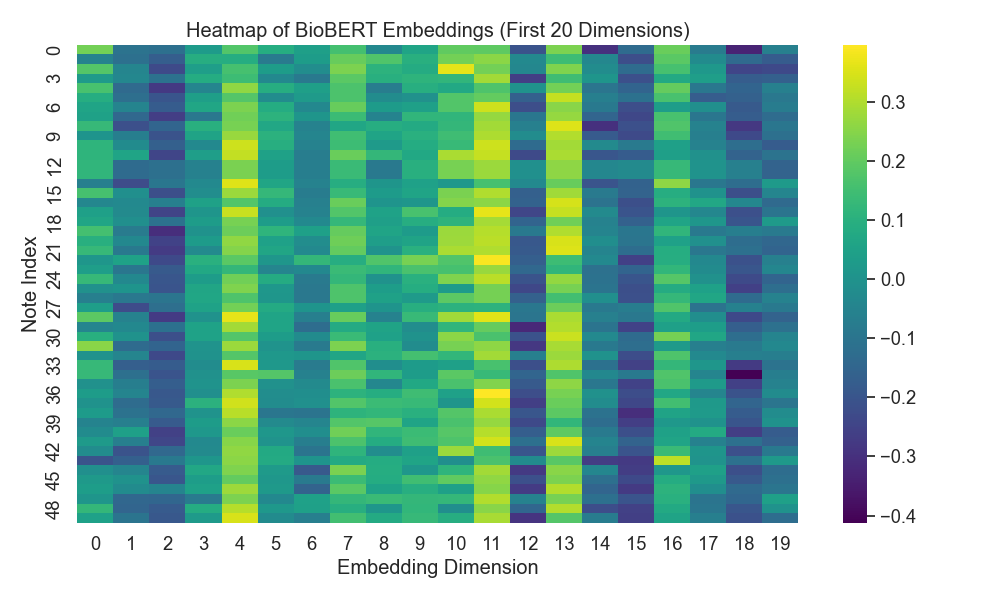
\includegraphics[width=0.8\columnwidth]{biobert_heatmap.png}
    \caption{Heatmap of BioBERT Embeddings (First 20 Dimensions). Values range from -0.4 to 0.3, reflecting note semantics.}
    \label{fig:biobert_heatmap}
\end{figure}

\begin{figure}[H]
    \centering
    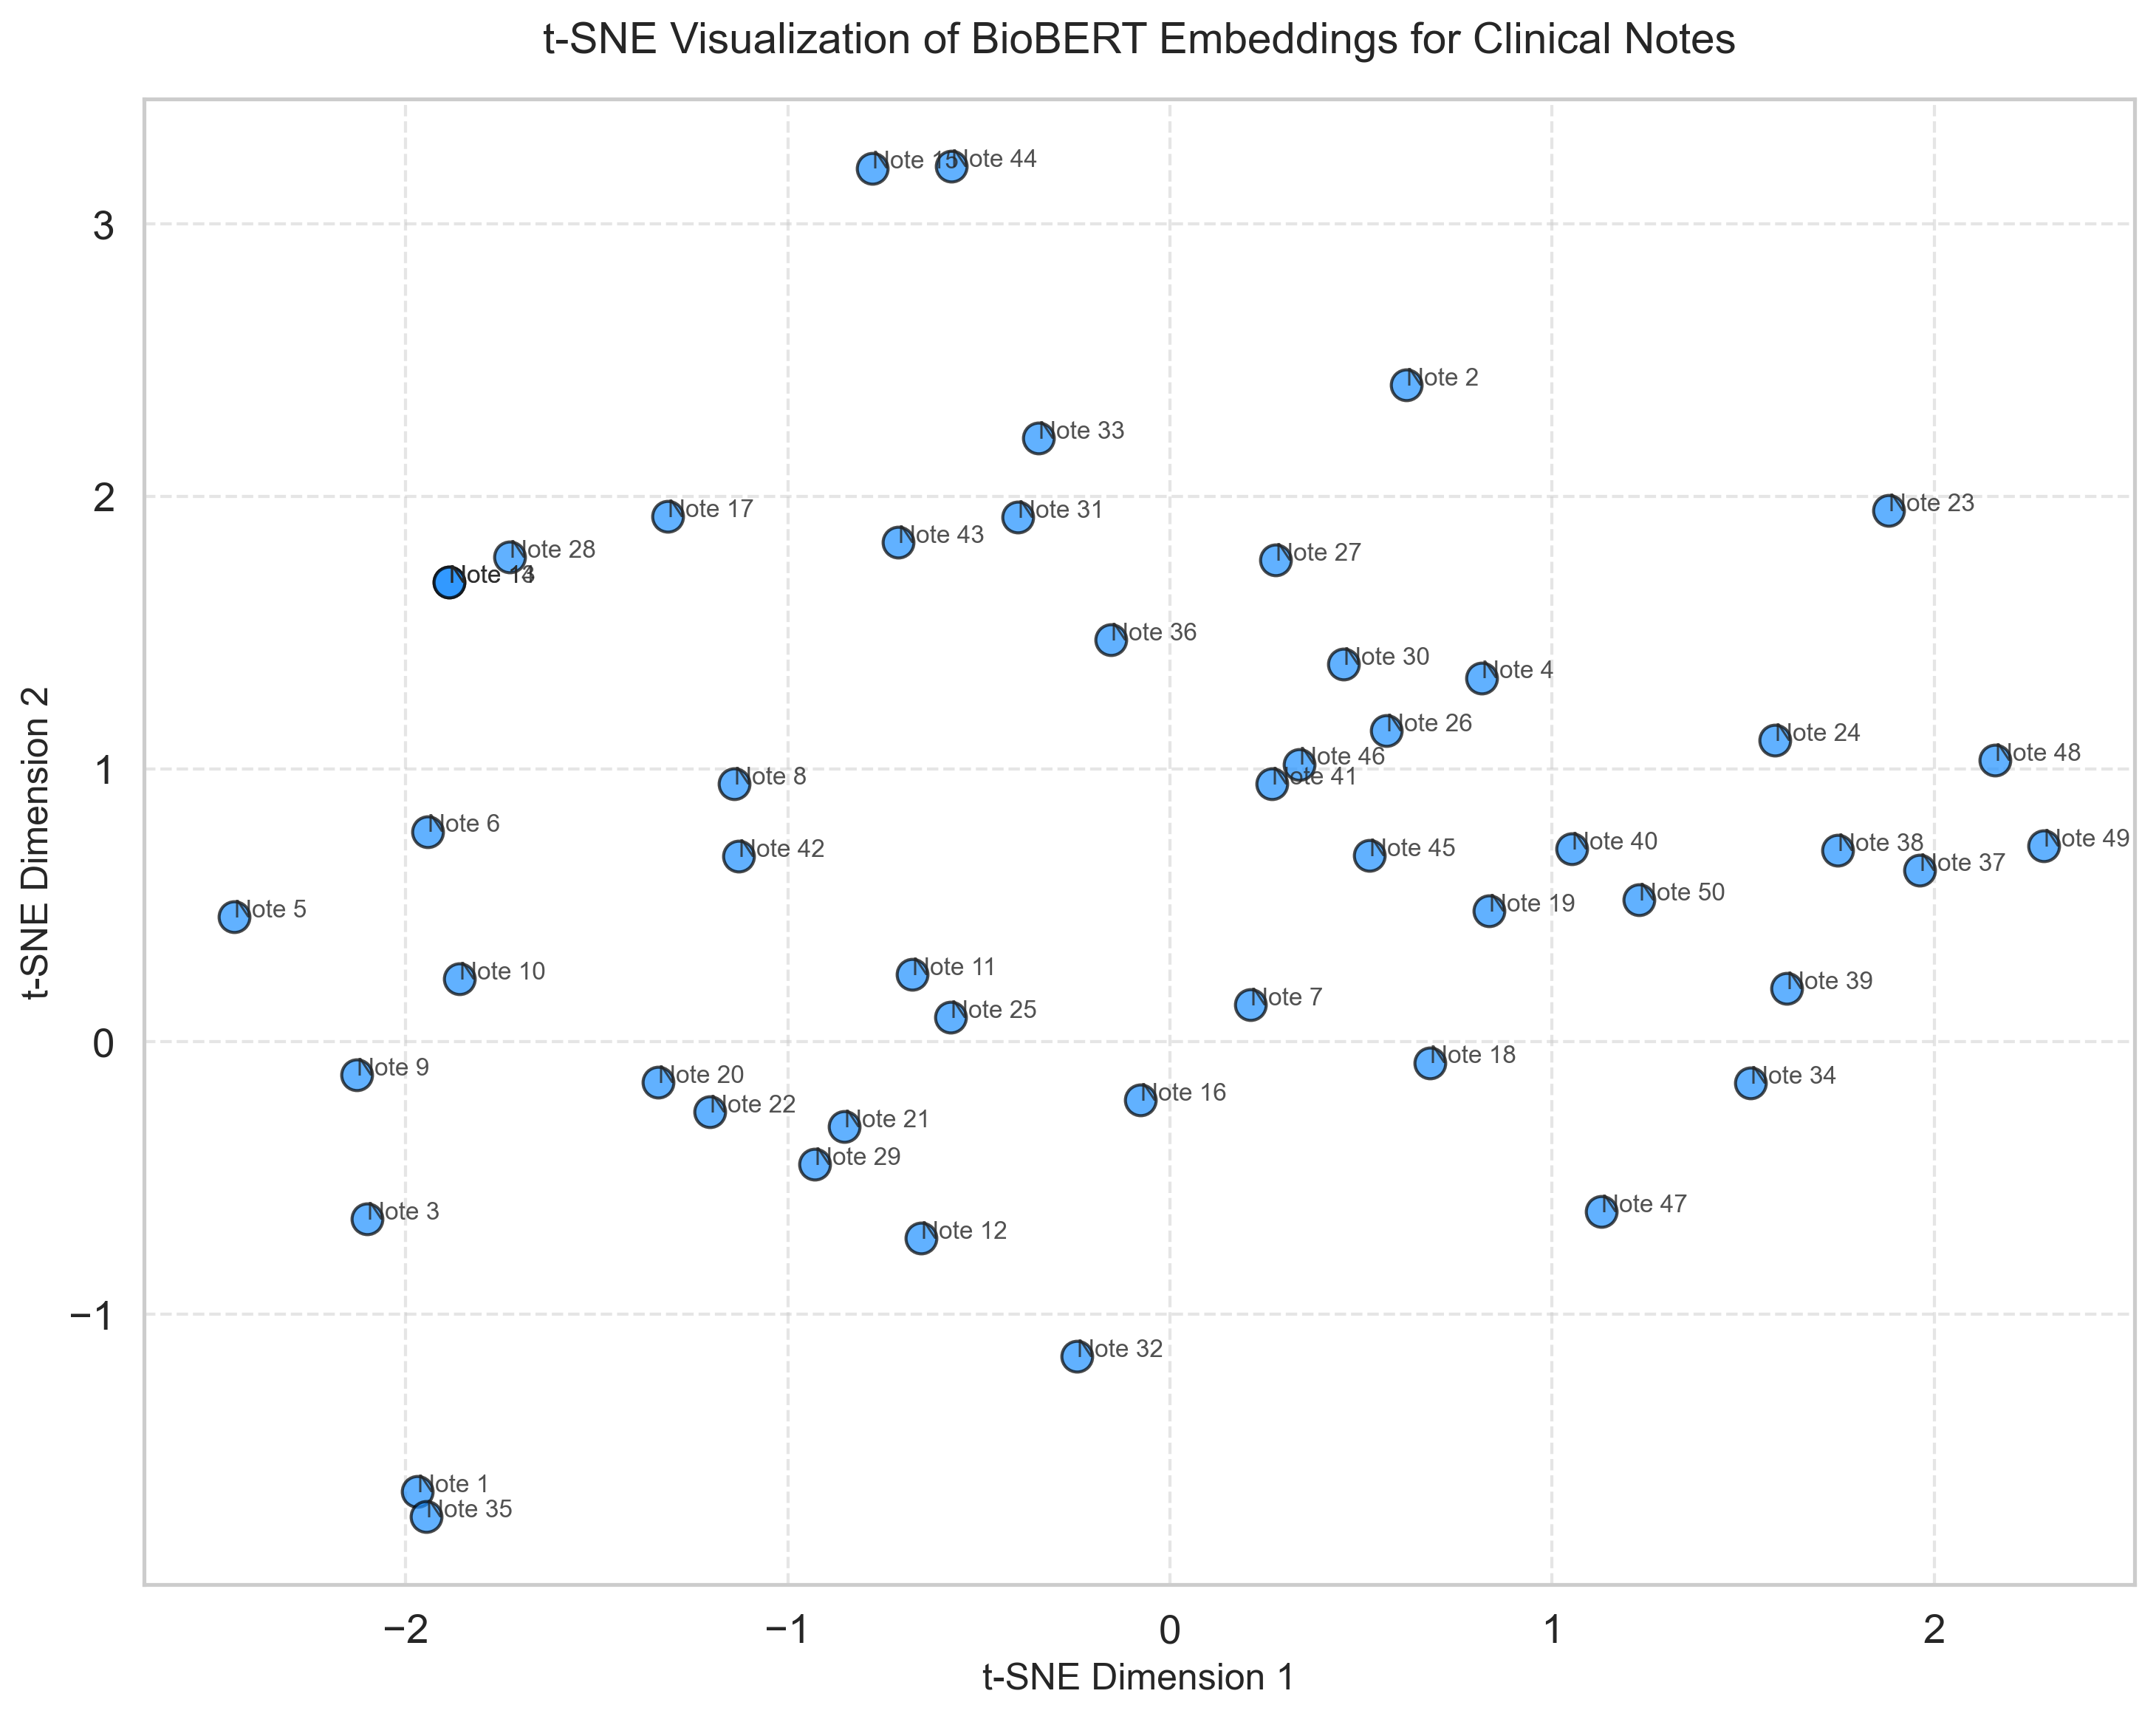
\includegraphics[width=0.8\columnwidth]{biobert_tsne_embeddings.png}
    \caption{t-SNE Visualization of BioBERT Embeddings for Clinical Notes.}
    \label{fig:tsne}
\end{figure}

\begin{figure}[H]
    \centering
    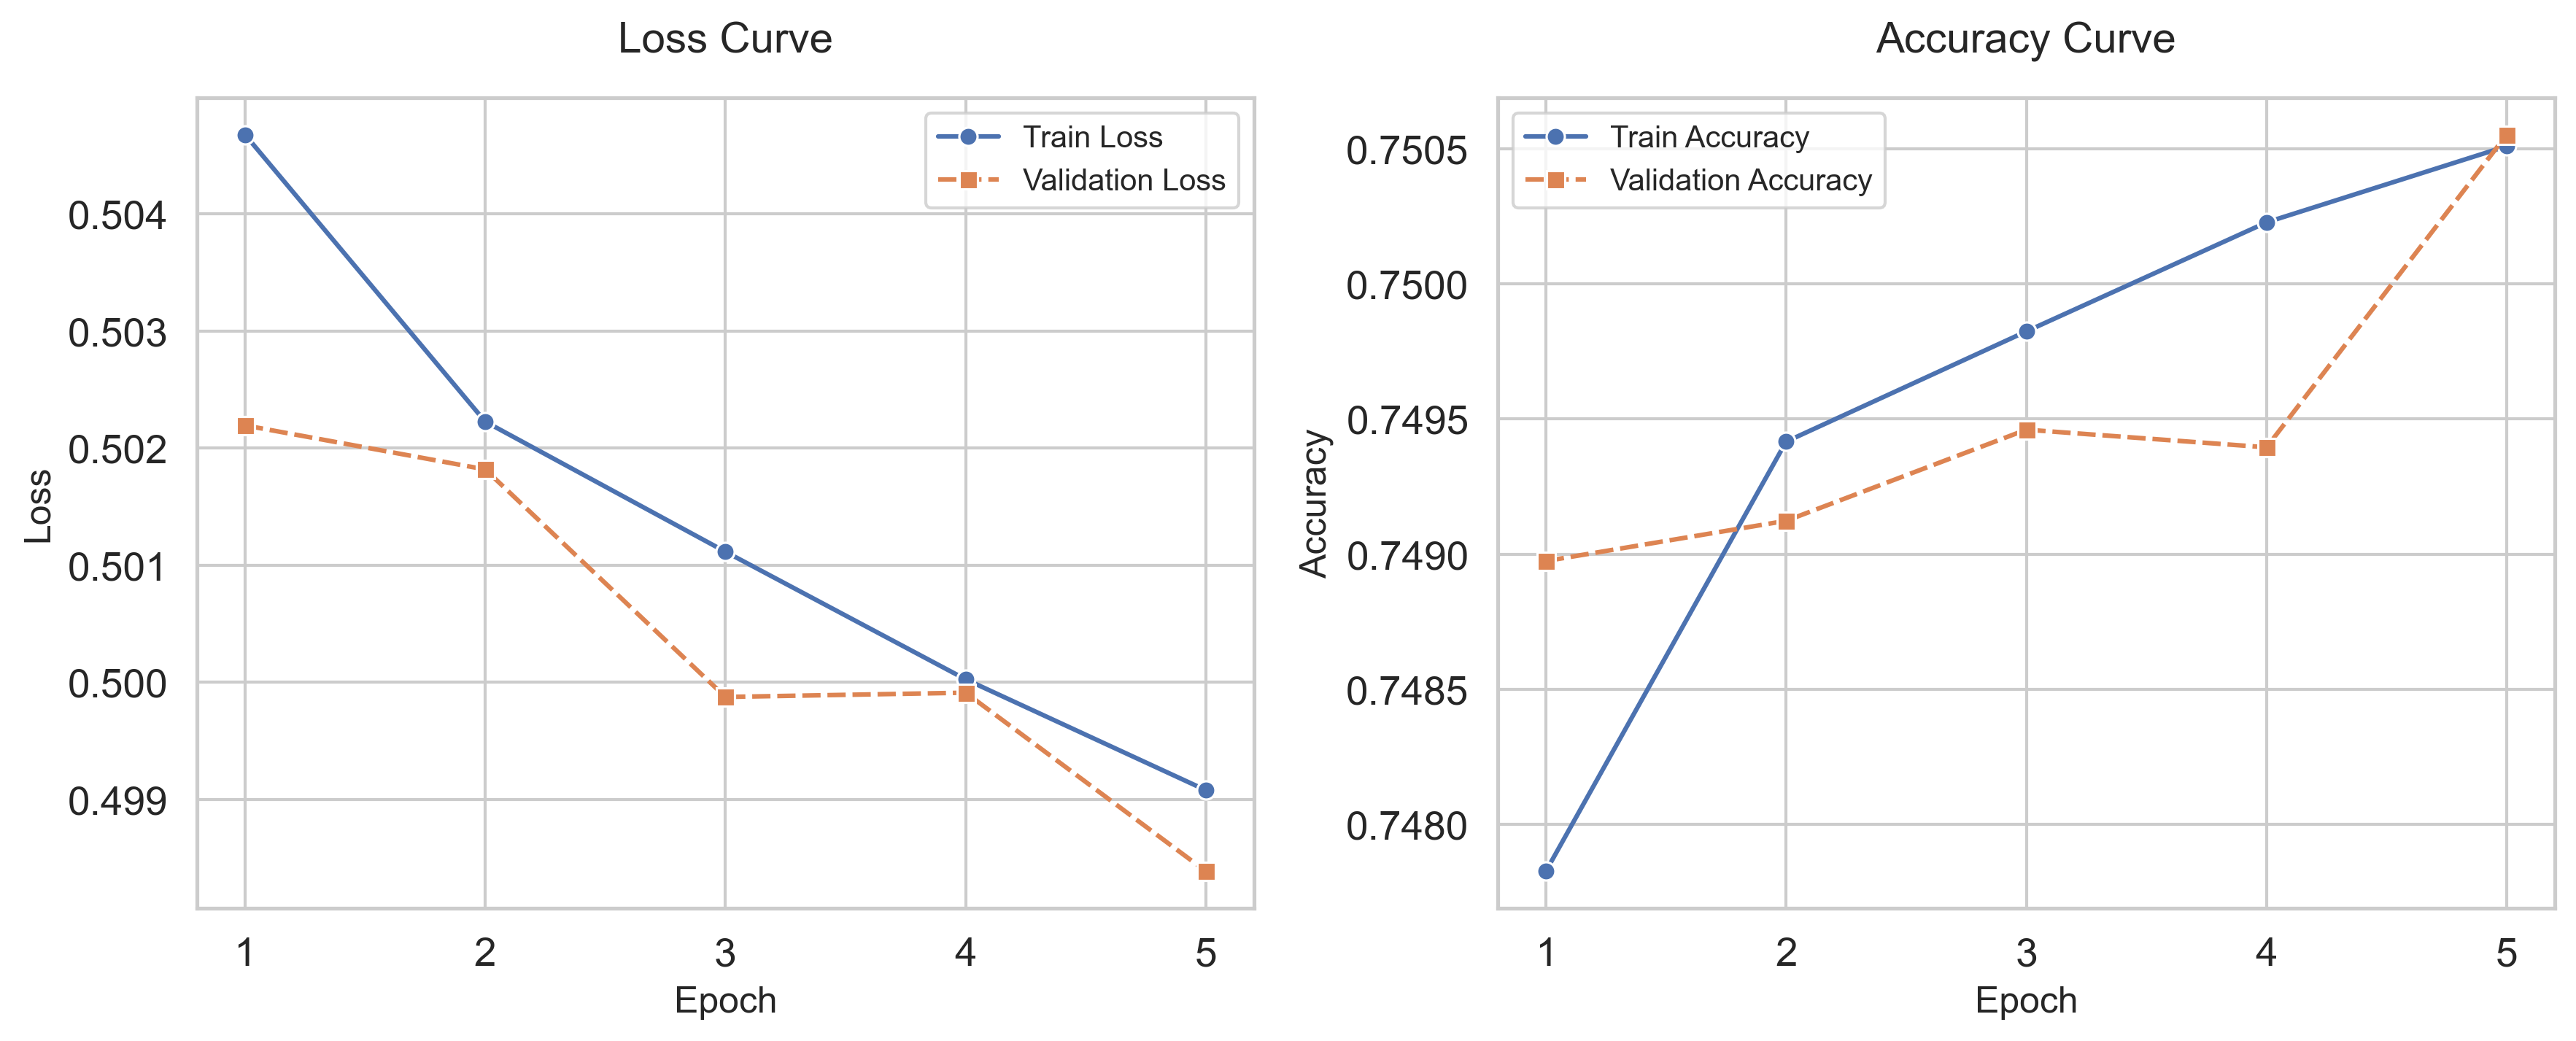
\includegraphics[width=0.8\columnwidth]{training_history.png}
    \caption{LSTM Training Results. Accuracy: Training 0.7505, Validation 0.7495; Loss: Training 0.500, Validation 0.502.}
    \label{fig:curves}
\end{figure}

\section{Conclusion}
A machine learning framework for early sepsis detection was developed, achieving an AUROC of 0.737 using LSTM and identifying heart rate and infection mentions as critical predictors. The integration of BioBERT embeddings with vital signs enhanced predictive performance, yet improvements in sensitivity and fairness are required. The t-SNE visualization in Figure \ref{fig:tsne} suggests that larger datasets or advanced models, such as GPT-4, could improve text analysis. SHAP results in Figure \ref{fig:shap} emphasize the significance of infection and fever, indicating a need for refined feature extraction. Fairness metrics in Figure \ref{fig:fairness} reveal disparities that necessitate broader demographic analysis, aligning with Yadgarov et al.’s advocacy for standardized methods \cite{yadgarov2024early}. Future efforts will employ SMOTE to address data imbalances and focus on real-time ICU monitoring, drawing inspiration from Hu et al.’s COMPOSER model, to facilitate swifter interventions \cite{hu2024impact}.

\bibliographystyle{IEEEtran}
\bibliography{references}

\end{document}